\documentclass{article}
\usepackage[utf8]{inputenc}
\usepackage{listings}
\usepackage{float}
\usepackage{natbib}
\usepackage{graphicx}
\usepackage{amssymb}
\usepackage{amsmath}
\usepackage{amsthm}
\usepackage{mathtools}
\usepackage{listings}
\usepackage{color}
\usepackage{hyperref}
\usepackage{ amssymb }
\usepackage{musicography}
%\usepackage[linesnumbered,ruled]{algorithm2e}
\usepackage{algpseudocode}
\usepackage{physics}
\NeedsTeXFormat{LaTeX2e}
\ProvidesPackage{quiver}[2020/11/27 quiver]
\newtheorem{theorem}{Theorem}[section]
\newtheorem{corollary}{Corollary}[theorem]
\newtheorem{lemma}[theorem]{Lemma}

% `tikz-cd` is necessary to draw commutative diagrams.
\RequirePackage{tikz-cd}
% `calc` is necessary to draw curved arrows.
\usetikzlibrary{calc}
% `pathmorphing` is necessary to draw squiggly arrows.
\usetikzlibrary{decorations.pathmorphing}

\definecolor{dkgreen}{rgb}{0,0.6,0}
\definecolor{gray}{rgb}{0.5,0.5,0.5}
\definecolor{mauve}{rgb}{0.58,0,0.82}

\tikzset{curve/.style={settings={#1},to path={(\tikztostart)
    .. controls ($(\tikztostart)!\pv{pos}!(\tikztotarget)!\pv{height}!270:(\tikztotarget)$)
    and ($(\tikztostart)!1-\pv{pos}!(\tikztotarget)!\pv{height}!270:(\tikztotarget)$)
    .. (\tikztotarget)\tikztonodes}},
    settings/.code={\tikzset{quiver/.cd,#1}
        \def\pv##1{\pgfkeysvalueof{/tikz/quiver/##1}}},
    quiver/.cd,pos/.initial=0.35,height/.initial=0}

% TikZ arrowhead/tail styles.
\tikzset{tail reversed/.code={\pgfsetarrowsstart{tikzcd to}}}
\tikzset{2tail/.code={\pgfsetarrowsstart{Implies[reversed]}}}
\tikzset{2tail reversed/.code={\pgfsetarrowsstart{Implies}}}

\lstset{frame=tb,
  language=Scala,
  aboveskip=3mm,
  belowskip=3mm,
  showstringspaces=false,
  columns=flexible,
  basicstyle={\small\ttfamily},
  numbers=none,
  numberstyle=\tiny\color{gray},
  keywordstyle=\color{blue},
  commentstyle=\color{dkgreen},
  stringstyle=\color{mauve},
  breaklines=true,
  breakatwhitespace=true,
  tabsize=3
}
\newcommand{\colim}{\operatorname{colim}}

\newcommand\rightthreearrow{%
        \mathrel{\vcenter{\mathsurround0pt
                \ialign{##\crcr
                        \noalign{\nointerlineskip}$\rightarrow$\crcr
                        \noalign{\nointerlineskip}$\rightarrow$\crcr
                        \noalign{\nointerlineskip}$\rightarrow$\crcr
                }%
        }}%
}

\newcommand\righttwoarrow{%
        \mathrel{\vcenter{\mathsurround0pt
                \ialign{##\crcr
                        \noalign{\nointerlineskip}$\rightarrow$\crcr
                        \noalign{\nointerlineskip}$\rightarrow$\crcr
                }%
        }}%
}

\graphicspath{ {./images/} }

\title{2MEME}
\author{Wyatt L. Meldman-Floch}
\date{11/27/2023}
\setlength{\parskip}{1em}

\begin{document}
\maketitle

\begin{abstract}
2MEME, a reputation model for p2p systems based on peer metadata and cryptographically secure hashes, is presented. It is dynamic, not relying on a set of trusted peers, and rotates the most accessible peers as leaders: those with the minimal entropy rate relative to all peers, or peers producing the most correct information. The core application and focus is optimizing consistency of a multi-layered consensus protocol. 

\end{abstract}

\tableofcontents

\setcounter{secnumdepth}{0}


\section{Introduction}
For a distributed system to maintain consistency (the C in the CAP theorem), it needs to optimize information gain and minimize discrepancies. One set of approaches rely on trust or reputation models to select between potentially conflicting updates from untrusted peers. There are many approaches to solving reputation problems in p2p networks. The most famous is Eigentrust, and many expansions upon the base framework, such as Honestpeer and Powertrust. Due to the curse of dimensionality they all employ some type of random walk to explore the search space of transitive trust between nodes, calculating a probability distribution via monte carlo integration over probabilistic scores of all peers, provided by each peer. These expansions typically focus on finding new features or representations of trust, such as in deepwalk or node2vec, which create an embedding of social data to normalize the edge weights of the peer graph.

This paper follows a similar approach using entropy or disorder across peer behavior and is specifically applied to a dag-based multi-layered consensus protocol. Whereas many approaches such as Eigentrust require a seed or whitelist of authority nodes to base trust upon, this is insufficient when requiring decentralization such as for distributed consensus networks like cryptocurrencies. 2MEME circumvents this by determining correctness without pre-trusted peers, allowing nodes to join and leave and preventing centralized control over consensus.

The core of the algorithm extends from the principle of maximal entropy, however applied in reverse. The maximum entropy principle states that new information added to a system increases disorder relative to the previous state of that system, proportional to novel information added. However, in the system architecture described below, the data structures themselves optimize the spread of incoming data via rumor based gossip such that discrepancies between peer state form cliques representing potential network partitions.

Periodically, a self avoiding random walk is performed on a graph of nodes representing peers and edges representing a vector of the entropy rate between data processed by each peer. The model chooses correct nodes according to a node influence metric based on 'availability', which is defined as the most strongly linked nodes; ranking the peers/nodes by how similar their proposals are as opposed to how diverse the total set of data is.

The goal of MEME is to improve upon PRO models by explicitly using an information gain metric to converge on an accepted state of a distributed system, via consensus.This achieves real elasticity comparable to elastic infrastructure like Elasticsearch and Elastic Map Reduce, as well as objective decentralization operating without potentially fraudulent human input.

\section{System Architecture}
The system considered here consists of a two layer consensus protocol, with two separate consensus processes, L1 and L0, directly influencing each other. Future work incorporating more consensus layers can be formulated using the Poincare Protocol and Protocol Topology specified in Blockchain Cohomology.

L1 peers perform a federated consensus of $O(\sum peers/3)$ complexity, converging on the state of each peer’s state cache. The contents of each state cache is a ledger of Addresses and collection of Transactions: data structures performing the transfer of a numerical amount (tokens) from one Address to another Address. Each Address has an associated linked list formed out of Transactions sent from this Address. The links are recursive cryptographic signature hashes between each sequential transaction at a discrete Ordinal.

Periodically, as each L1 node reaches the limit of its mempool or in response to a timed trigger, they initiate a consensus process, acting as an ‘owner’ peer, which selects two ‘facilitator’ peers to share its state cache with. The two facilitator peers also share their state cache with each other and then the owner peer. The output of this process is a data structure, signed by the owner and facilitators, called a ‘block’ which consists of each peer’s state cache data and two ‘parent edges’ called Tips, which are hashes of previous blocks; the end result is a triangle, where two corners are tips and the third is the new block. This can be conceptualized as a ‘triangulation of state’ which forms a forward arrow of time out of parallel-process state transition data. This is realized as a data structure called the ‘Data Dependency Graph’ which is a directed acyclic graph of blocks with two parent edges, and three dimensions; namely, height, width and depth. 

These blocks constitute a directed acyclic graph called the Data Dependency Graph and their contents form a ledger of Addresses. Both of these have a poset topology, from which the forward arrow of time can be constructed out of parallel events. Each block is then spread across all L1 and L0 peers via rumor based gossip, so that they can be used as ‘Tips’ to form edges between old and new blocks.

Tips and facilitators are selected using a pure function that seeks to maximize the area (in terms of height, width and depth,) thus increasing the potential parallelism by enforcing consistency across all peers. L1 nodes are pruned according to an entropy calculation by L0 nodes on their blocks created; each block is created deterministically according to the total set of tips and peers, deviations from this result in low trust (and rewards). L1 trust scores are then normalized between 1 and -1 with low trust outliers being removed and addresses temporarily blacklisted.

Data contained in the L0 peer's mempool consisting of L1 blocks, is spread amongst L0 peers via rumor based gossip with $O(log(\sum peers))$ complexity, converging the state of each peer to the union of all peers'. Periodically, as the Data Dependency Graph reaches new heights or on a timed trigger in case of low network traffic, each L0 peer proposes a Snapshot to its L0 peers using rumor based gossip. The contents of these Snapshots are L1 blocks, and a parent reference, formed out of recursive cryptographic signatures, to the peer’s previous Snapshot proposal. This forms a sequential/poset topology for L0 peer proposals like for Addresses. At each ‘Height’ step, one proposal is selected from the set of all proposals, deemed the Majority Snapshot. The Majority Snapshot is chosen as the count of occurrences within the set of proposals, multiplied by the node influence or sum of trust scores of each peer that proposed it. 
	
Periodically, at an interval multiple of snapshot height called height-diff interval, the L0 nodes cycle between ‘active’ and ‘passive’ states. The total number of active L0 nodes is equal to $\sqrt{\sum peers}$, thus the total complexity for ledger state convergence (known as finality time) is $O(\sqrt{\sum peers}^2) = O(\sum peers)  = O(n)$. Peers are cycled each interval according to deterministic locality sensitive hash collisions between the last snapshot hash and all the L0 peer addresses that have not been blacklisted. Rewards for each round are proportional to the cumulative sum of information gain (inverse of entropy rate) reported by L0’s peers and low trust outliers are blacklisted temporarily 

In both L0 and L1, a 'double spend' or submission of invalid data as valid, with the attempted result being the attribution of new tokens to some Address, the node Address's balance is reduced to 0 in a process known as 'slashing'.

\section{Minimizing the Entropy Rate}
Information gain can be formulated as the reduction of entropy or disorder in a dynamical system and depending on the characteristics of the system, it is calculated in one of many ways. For the purposes of 2MEME, which is formulated for application to consensus networks, it is calculated as a stochastic process.
	A stochastic process is an indexed sequence of random variables that do not need to be independent or identically distributed. In a consensus network, each peer continuously proposes variable state data, converging on an accepted state according to the rules of the consensus algorithm. This state data, in our case called blocks, can be independent or dependent on each other; and the amount of blocks as well as the specific blocks proposed can fluctuate or differ completely. Each block has an indexed order, or in the case of the system architecture above, a poset topology; meaning that they are strictly ordered. Thus these distributed systems fulfill the requirements of a stochastic process and can be modeled as such. While it is possible to apply MEME to linear blockchain protocols, it was formulated specifically for use in the system architecture above, with three indices: height, width and depth. The following formulas are specific to this poset topology.
	Consider a set of peers $N = (n_0 …n_i)$, acting as random variables which produce outputs $O = (o_{0,0,0} … o_{h,w,d})$, such that $h<w$ and $w>d$, the system has a strict order given by poset topology. These indices can be reduced to discrete indexes, such that each index, there is a binary value representing each node proposing a specific block or not. This is calculated using following formula for join entropy (see ref 3) 
	
\begin{equation}
H(X_1, \dots, X_N) = -\sum_{x_1 \in \chi_1} \dots \sum_{x_n \in \chi_n} P(x_1,  \dots, x_n) log_2 [P(x_1, \dots, x_n)]
\end{equation}
	
	the limit of which as h, w, d approaches infinity gives the entropy rate.
If a block index contains each node, then the specific block has entropy of 0. If it contains $|n| < N$, the entropy is $> 0$. Conversely, if nodes propose blocks such that their indices conflict with other proposals, they contribute to the overall disorder in the system. Proposed blocks with valid yet duplicated data, contribute to overall disorder as well. Thus the state with the minimal entropy can be considered the greatest common subset of all proposed blocks, and entropy calculated as deviation from the greatest common subset. Note that in the case of graph partitions that are not within this subset, yet still contain valid data, the data should still be contained within the overall state transition, however the node that only processed it’s lone subset can be considered faulty in terms of consistency and partition tolerance (CAP.) In order to promote consistency, a rumor based gossip algorithm propagates blocks, calculating signatures upon them and for use as Tips, to optimize for a maximal subgraph of peers to accept the block and propose it within its Snapshot. This prevents several sybil attacks such as lie and wait and ddos, by attempting to create the longest signature chain as possible, i.e. the largest common subset; nodes attempting these types of attacks are identified via independent subsets and/or invalid blocks.

Finally, the inner product of entropy rates are used to construct a feature space $F$ before passing into the random walk below (first part of 2MEME)

\begin{equation}
F = \sum_i \lambda \ket{p_i} \bra{p_i}
\end{equation}

where $\lambda$ is a normalization function that maps the sum to between -1 and 1.

\section {Permissionless vs Permissioned approaches}
Two algorithms for gathering entropy data are presented below. The key difference is the rate and method of gathering entropy rate. The first enforces a service level agreement requiring each peer to train its model at the same rate, achieving greater determinism and enabling a token reward model for an open network. In the batch model, at every snapshot height-diff interval, each peer proposes a new predicted trust vector within their proposals. They are then used to weight peer proposals for majority snapshot calculation until snapshot height-diff interval +1.
The second, online algorithm, is a greedy approach that reduces the in-memory cost of running each peer’s model on a deterministic schedule albeit at the loss of determinism that would allow a fair token reward model. It is more suited perhaps to applications that can relax determinism for  open network rewards to focus on elasticity. The online algorithm periodically gossips predicted trust vectors to peers over the Peer api endpoint (“~/trust”), which are then cached and fed into the TrustManager on a time based periodic interval.

\caption{Batch Algorithm (permissionless): Entropy Rate (Optimal for node rewards/cycling between active and passive nodes)}\label{alg:cap}
\begin{algorithmic}
\Require $h, i \in \mathbb{N}$
\Require $H \ggg  i$
\State $h \gets H$
\State $n \gets N$ \Comment{these are nodes}
\For{$h \gets H$}
\If{$h \bmod i-1 == 0$}
    \State $state space = entropy(N)$ \Comment{Entropy rate relative to GCS}
    \State $probability space = walk (state space)$  \Comment{Montecarlo method}
    \State send encrypted scores to peers

\Else{$h \bmod i-1 == 0$}
    \State send unencrypted scores to peers
    \If {$valid(n) \forall n \in N$}
    \For{$n \gets N$}
   	 \State update scores for peers
	 \State update active and passive peerlist

\end{algorithmic}
\end{algorithm}

\caption{Online Algorithm (permisioned): Approximate Entropy Rate (current implementation, optimal for minimal resource usage, training model over shorter periods should help output, spamming results/sybil collusion should be detected by model, good test)}\label{alg:cap}
\begin{algorithmic}
\Require $h, i \in \mathbb{N}$
\Require $H \ggg i$
\State $h \gets H$
\State $n \gets N$ \Comment{these are nodes}
\For{$h \gets H$}
\If{$h \bmod i == 0$}
    \State $state space = entropy(N)$ \Comment{Entropy rate relative to GCS}
    \State $probability space = walk (state space)$  \Comment{Montecarlo method}
    \State send encrypted scores to peers
    \State update scores for peers
    \State update active and passive peerlist

\end{algorithmic}
\end{algorithm}


\section{Monte Carlo simulation: estimation via self avoiding random walk}
Next a self-avoiding walk is employed to perform community detection, the output of which can be used to calculate availability and node influence. Note, to avoid confusion between a consensus network and graph, nodes are called servers below.

The output of the entropy rate calculation is a graph, with a server’s peers corresponding to nodes and edges as the relative joint entropy between the server and its peers. The edges are a ‘view’ of the performance of each peer relative to itself. This is passed to the TrustManager, a background process that performs a self-avoiding random walk across the graph of nodes connected by relative joint entropy and outputs a vector containing a trust score for each node relative to the server hosting running the process (predicted trust).

The self avoiding walk is performed by the method runwalkfeedbacksinglenode, which performs a series of feedback rounds, walking on the input graph and adjusting the edge weights between nodes for each successive round. The total number of feedback cycles are configurable and in general the larger number of cycles has a more accurate output, albeit at the cost of increasing resource intensity. The configurations are batchIterationSize and maxIterations. On each batch iteration a random path length from a random number generator (between 1 and total nodes) is chosen and then passed to the walk. The walk goes through and only walks on positive edges (relative entropy scores are normalized between -1 and 1), keeps track of nodes visited so far, then the sampling function determines the next neighbor to walk on. This is determined according to the normalized probability (via method normalizedPositiveEdges), such that the positive edge subset sum up to one.

As this iterates, transitive trust scores are added, because products of trust are quite small. However, over many iterations they sum, to large numbers which is better for differentiating between scores. The main walk function walk() gets invoked by walkFromOrigin() inside runWalkRaw() which iterates over numIterations, adding up the scores into val walkScores for each node, removing the server’s own. After that function is called, one “batch” has been created. 

Finally there is batch convergence in runWalkBatchesFeedback. This converges when a delta variable, which is just root mean squared error, becomes less than or equal to an epsilon variable, where epsilon is set to 1e-6; i.e the function terminates when scores don’t change between batches by one part in a million. The output of the walk, batchScores, is not normalized, so they are renormalized by the Normalize function between each iteration until convergence.

One difference from similar models is the incorporation of negative scores. After the batches are performed, it explores the negative scores (val negativeScores) of nodes that it trusts (positive outputs of the walk). On the first cycle, the model only reaches nodes with positive transitive trust, which can be considered the most influential servers. These most influential servers are relative to the host server, and the servers they distrust have their scores down weighted. The positive scores and negative scores are added, then weighted by how influential the server proposing these scores is. They are weighted such that its negative edge trust quantity*(influential node’s score/numNegEdges), after that they are all normalized via renormalizeAfterNegative. Output, $P_i^h$ is defined as follows.

Given a source node $i$, suppose it is possible to reach $N_i(h)$ different nodes performing walks of length $h$, departing from $i$. Then we say that $i$ has $N_i$ neighbors at a distance $h$. Each neighbor is reached with a different probability, which is represented by the vector $P_i^h = \{ P_1^(h) \dots P_{N_i(h)}^(h)$
	
	
\begin{equation}
k(h) = \exp (-\sum_j p^{h}_j log p^{h}_j )
\end{equation}

\section{Classification logic}
Now we have a manifold of node influence, we can look for signals between sybil and non-sybil nodes and build a classifier. The classifier defined as follows simply looks at the first three eigenvectors and their eigenvalues to identify sybil nodes. Its quite possible to improve upon the experimental results using a differential equation solver as provided in tensorfow or pytorch, which would be able at least incorporate higher order terms if not catch hidden nonlinear signals

First a new vector consisting of the successive diffs, normalized between 0 and 1, between all elements in $P_i^h$ is calculated, namely $d_i^h$ which has $dim(i, h-1$ then generate a manifold from it's self-tensor

\begin{equation}
d_i^h \oplus d_i^h
\end{equation}

calculate the principal components (eigenvectors sorted by highest eigenvalue), $\lambda_1, \lambda_2 ,\lambda_3$ as well the 'max plane' $p_i$, similar to the 'top hat' in signal/fourier analysis but with a flat top (all diffs are within a threshold of the mean $\mu$) which is the index range in $d_i^h$ with the highest values, the 'right bias' $b_r$ and 'left bias' $b_l$ which are the ration of total sum of values to the left of $p_i$ divided by total scores and  total sum of values to the right of $b$ divided by total scores respectively. Finally consider 'population diffs' 

\begin{equation}
\lambda_{pop} = 1-(\lambda_{i-left}/\lambda_{i-right})
\end{equation}
where $1-(\lambda_{i-left}/\lambda_{i-right})$  are the population or number of nodes contained within biases calculated from each of the principal eigenvalues.

Now, there are five scenarios to determine non-sybil nodes: first if the max plane maxes up over $20\%$ of the distribution and either biases are less than $60\%$ of the distribution, return the biases as non-sybil nodes. Second, if either the absolute value of the ratio of mean to population valiance is < $1x10^{-17}$ or the difference between the absolute value of the first principal component and the  absolute value of the second principal component is greater than the population standard deviation by $30\%$, return the entire set of $P_i$. Third, if the difference between the principal and second principal eigenvector is greater than the population standard deviation by $20\%$ or the minimum population diff (of all 3) is the population diff of the maximum principal component, then if the difference between the absolute values of the population biases of the principal eigenvalue $|\lambda_{left}| - |\lambda_{right}|$ is greater than the pupulatino standard deviation, return the right bias of the max principal component; if only the first condition is true, return the left bias of the max principal component. Next he same logic is then applied for the second and third principal components. 

Finally, if the total non-sybil nodes to be returned are less than $10\%$ of the population ($90\%$ identified as sybil), return the entire set of nodes.


\section{Experimental results}
The following results were generated from a simulation involving 100 node instances. Several sumulations were run for various types of attacks, which will be outlined below, and with varying percentages of nodes all acting in unison from 0 to 100 in 20 percent intervals. Each type of attack can be reduced down to sybil nodes reporting scores of themselves or non-sybil nodes according to a distribution i,e low scores for non-sybil or high scores for sybil nodes. In the following visualizations, each attack type occurs on the y axis, the sybil percentage is given by the x axis and the z axis is the f-score of the model.

Note that many different scenarios are tested within unit tests and the symulation framework, however a subset based off of the actual protocol's implementation (whithin which this model is used) are 

The attacks tested are as follows:

organicDistroDir: no attack, organic behavior from each node

symmetricSybilOne/Sybil nodes forging their scores as 1.0: all sybil nodes git each other the max value in their proposal

symmetricNegOne/Sybil nodes forging their scores as -1.0: all sybil nodes choose min value for each other in their proposal

symmetricZeroSybil nodes forging their scores as 0.0: all sybil nodes choose 0


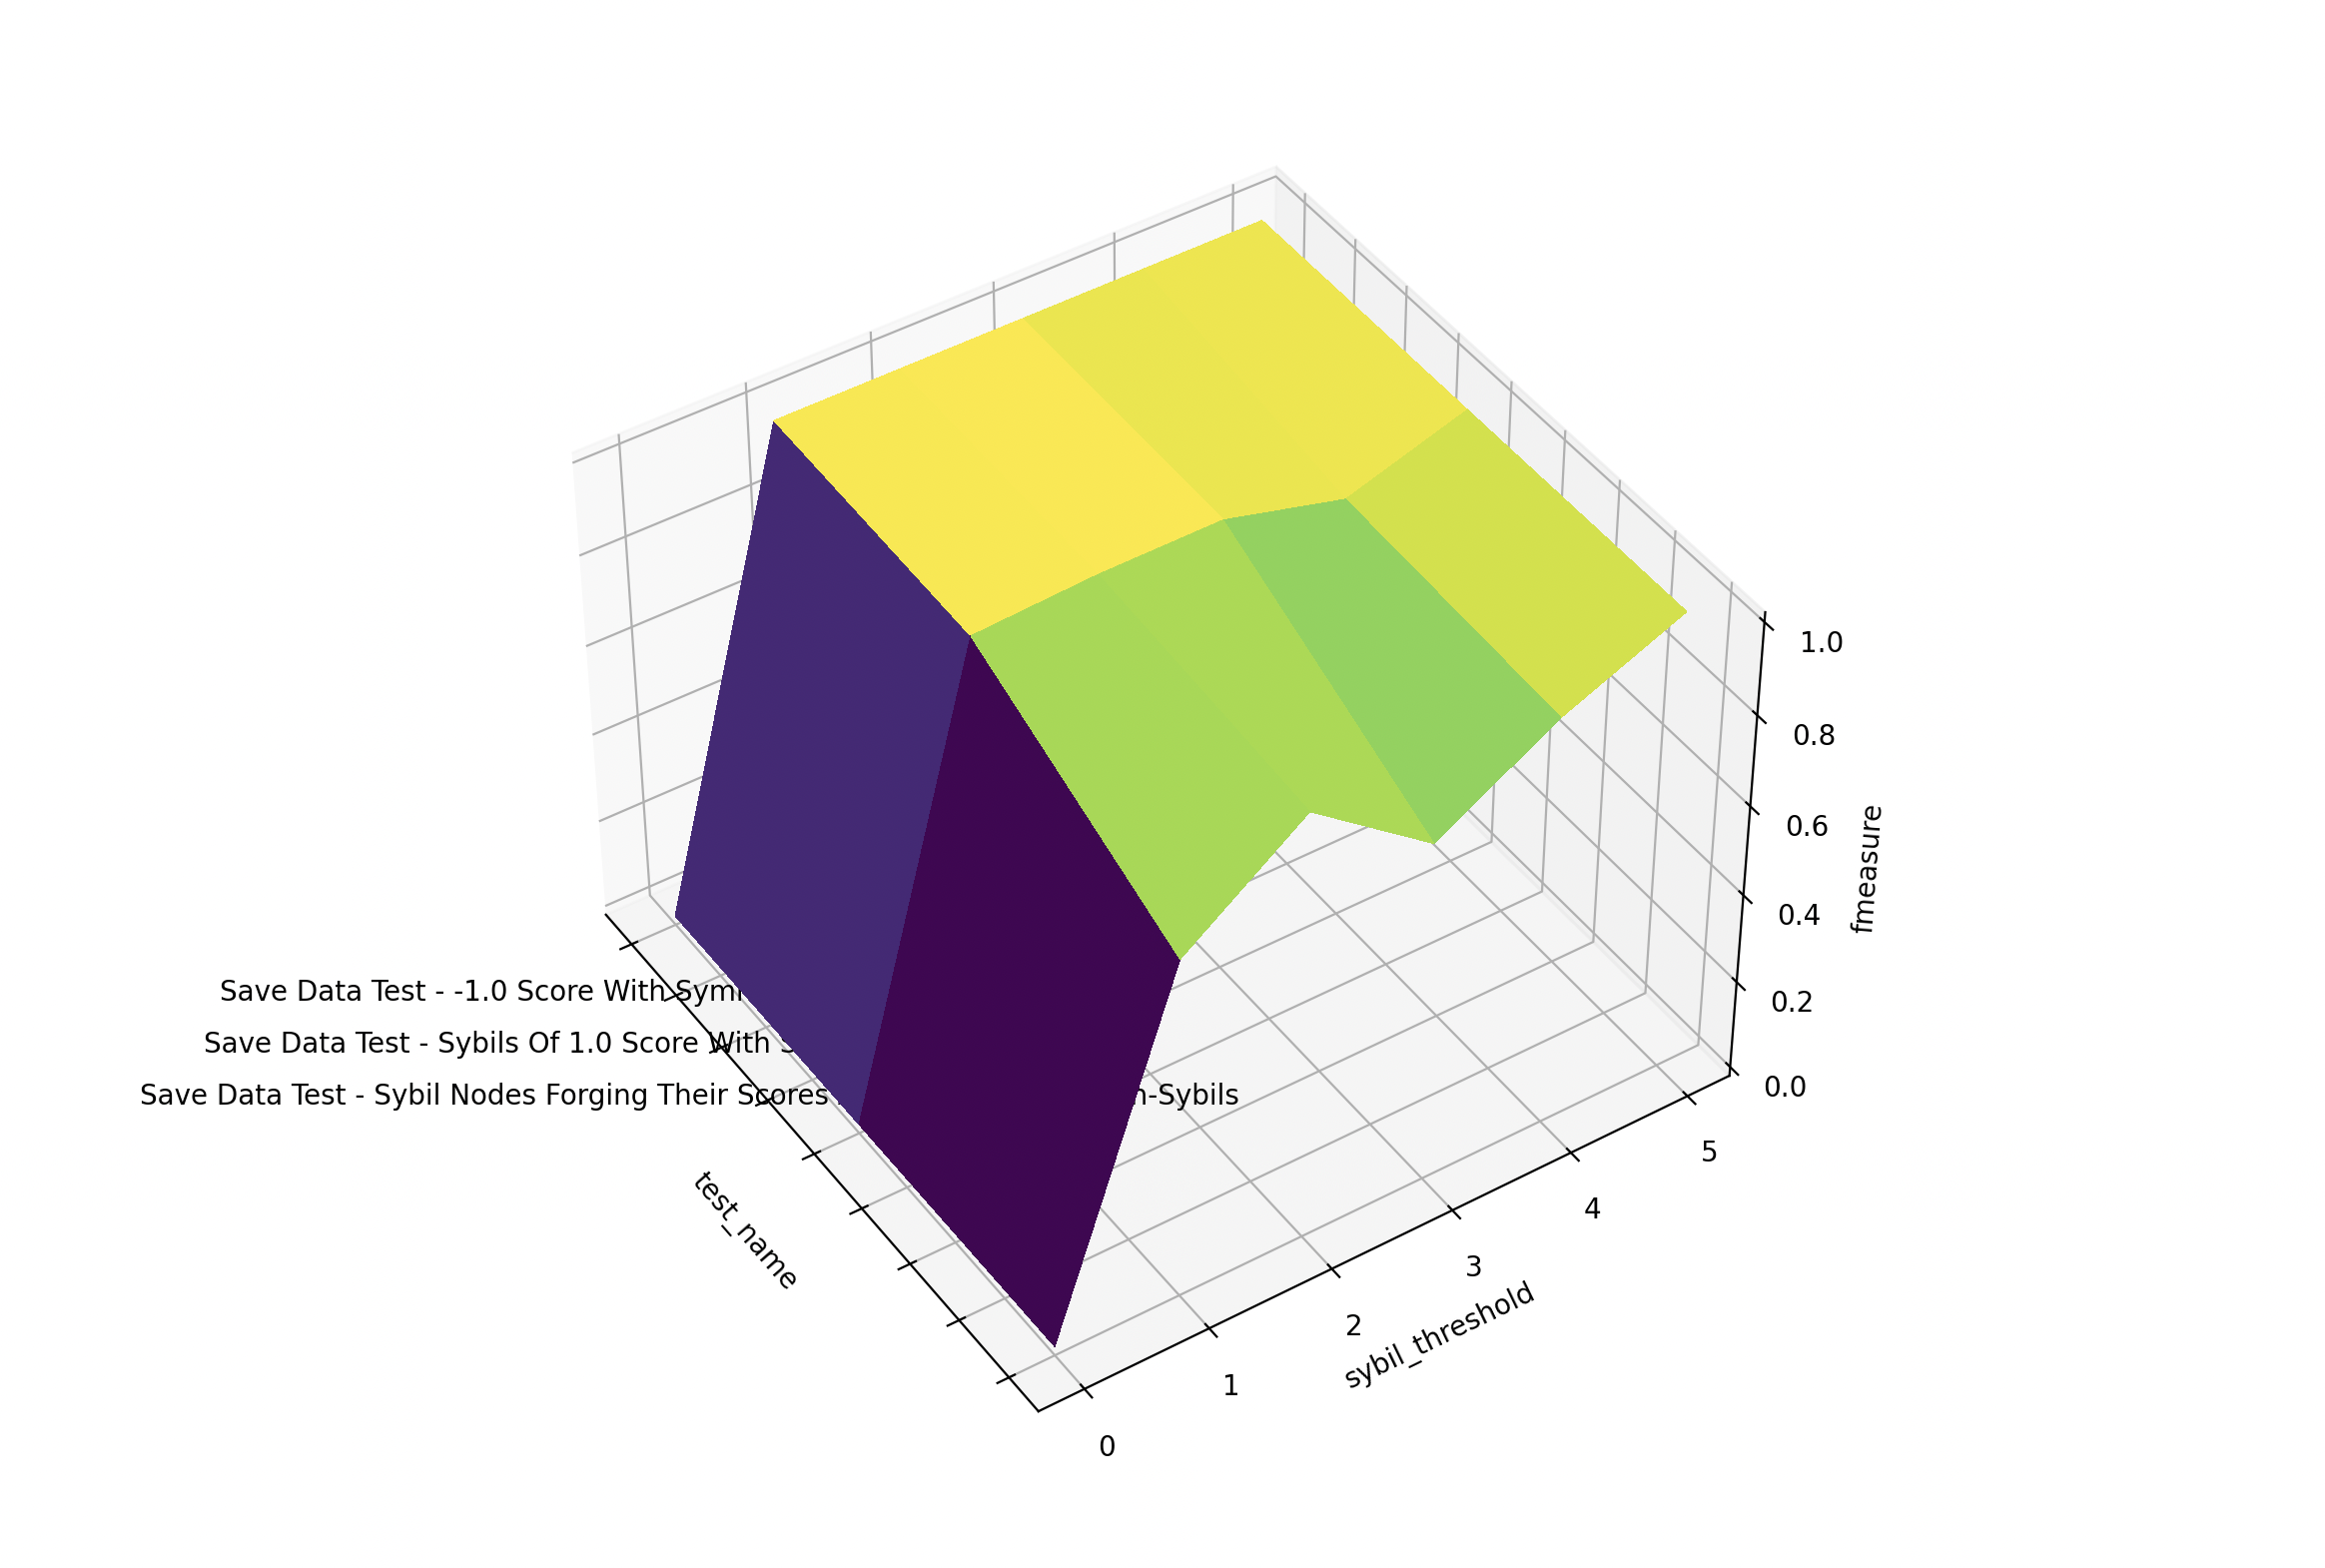
\includegraphics[width=\textwidth, height=\textwidth]{f-score-surface-plot}
Here we have a surface plot of fscore according to attack and sybil threshold. As we can see, the most effective attach is for sybils to self report scores of 0.0, yielding an f-score of ~0.7. This is still a solid score for any model and compared to existing consensus models which have an fscore of 0 for sybil percentages above 50 percent, is remarkably successful and provides a huge comparative advantage.


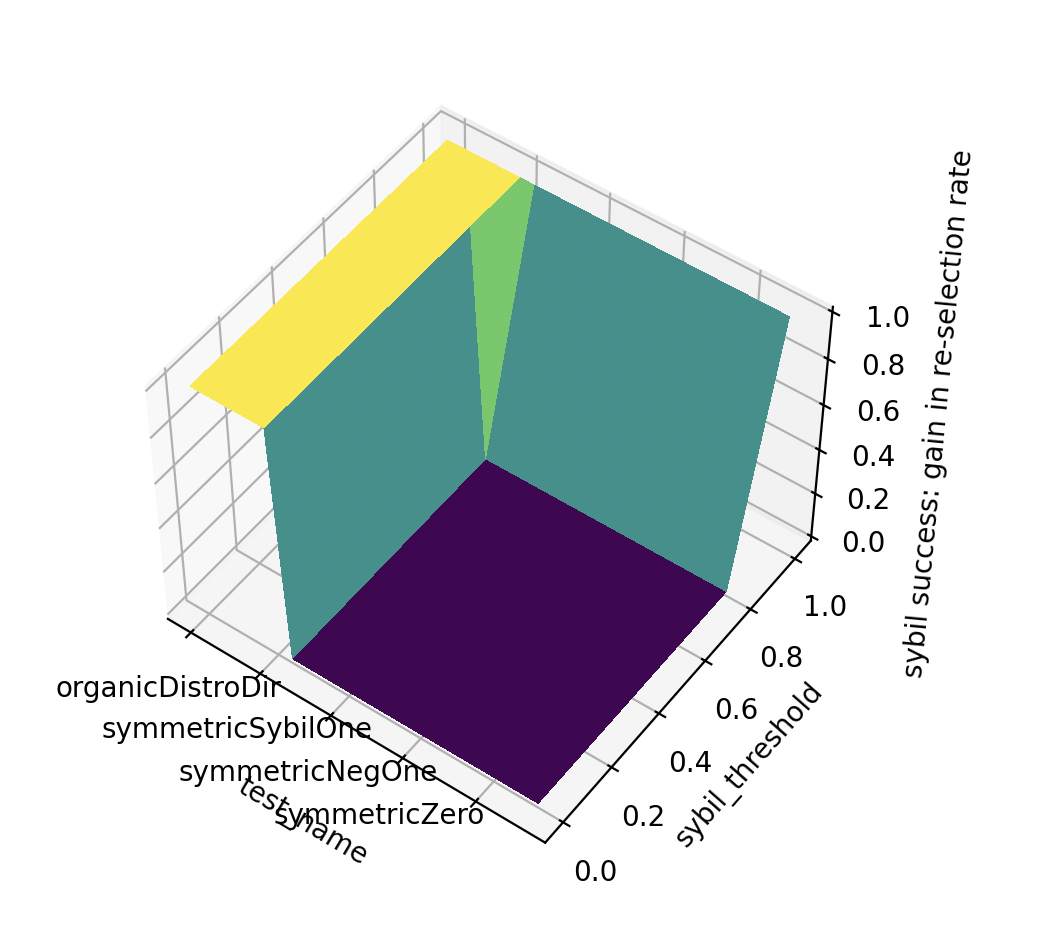
\includegraphics[width=\textwidth, height=\textwidth]{attack-success-suface-plot}
Here we have a plot of the difference between nodes cheating and not cheating. The vertical axis is an the percentage of nodes selected for consensuls, vs actually submitting scores based upon the true entropy rate. The ledge on the top left ("sybil" set doesn't cheat) as well as the $100\%$ sybil case on the right, shows $100\%$ of sybils selected for next round. 

\section{Further investigation}
	Modifications to the self-avoiding walk implementation could yield positive effects. As in many monte carlo integrations, the direction chosen at each step could be chosen according to a distance metric as opposed to randomly. Albeit, at the computational cost of increasing the dimensionality the trust graph’s edges as well as in-memory expense of the metric calculation. Notably, this approach was employed by (N. Koroviako) who used jaccard similarity to define trust out of relationships between review texts; as 2MEME approach focuses on information gain, it would follow to select the next path at each step based on minimizing entropy rate of second order proposals (each edge would contain raw proposals, and choose the next node that has the minimal entropy rate compared to the current’s proposals.)
	Use Hausdorff clustering to identify/embed hierarchies, could lead to a shared security model. Could have applications in further anomaly detection extending to higher dimensions of entropy in tandem with graph embedding or deep learning approach.
	
	



\bibliographystyle{plain}
\begin{thebibliography}{9}
\bibitem{latexcompanion} 
Baez, John C
\textit{Circuitry, EE and chain complexes}.
\\\texttt{https://math.ucr.edu/home/baez/week288.html}

\end{thebibliography}
\end{document}
